\section{Managing different size and filters}

Scaling down an image reduces not only the size but also the details of the image. This can be seen in figure \ref{fig:task5}. While with scale factor of 0.5 we can still appreciate most of the details of this particular image, after rescaling it to 0.01 the original size almost all details are lost.

\begin{figure}[!hbt]
  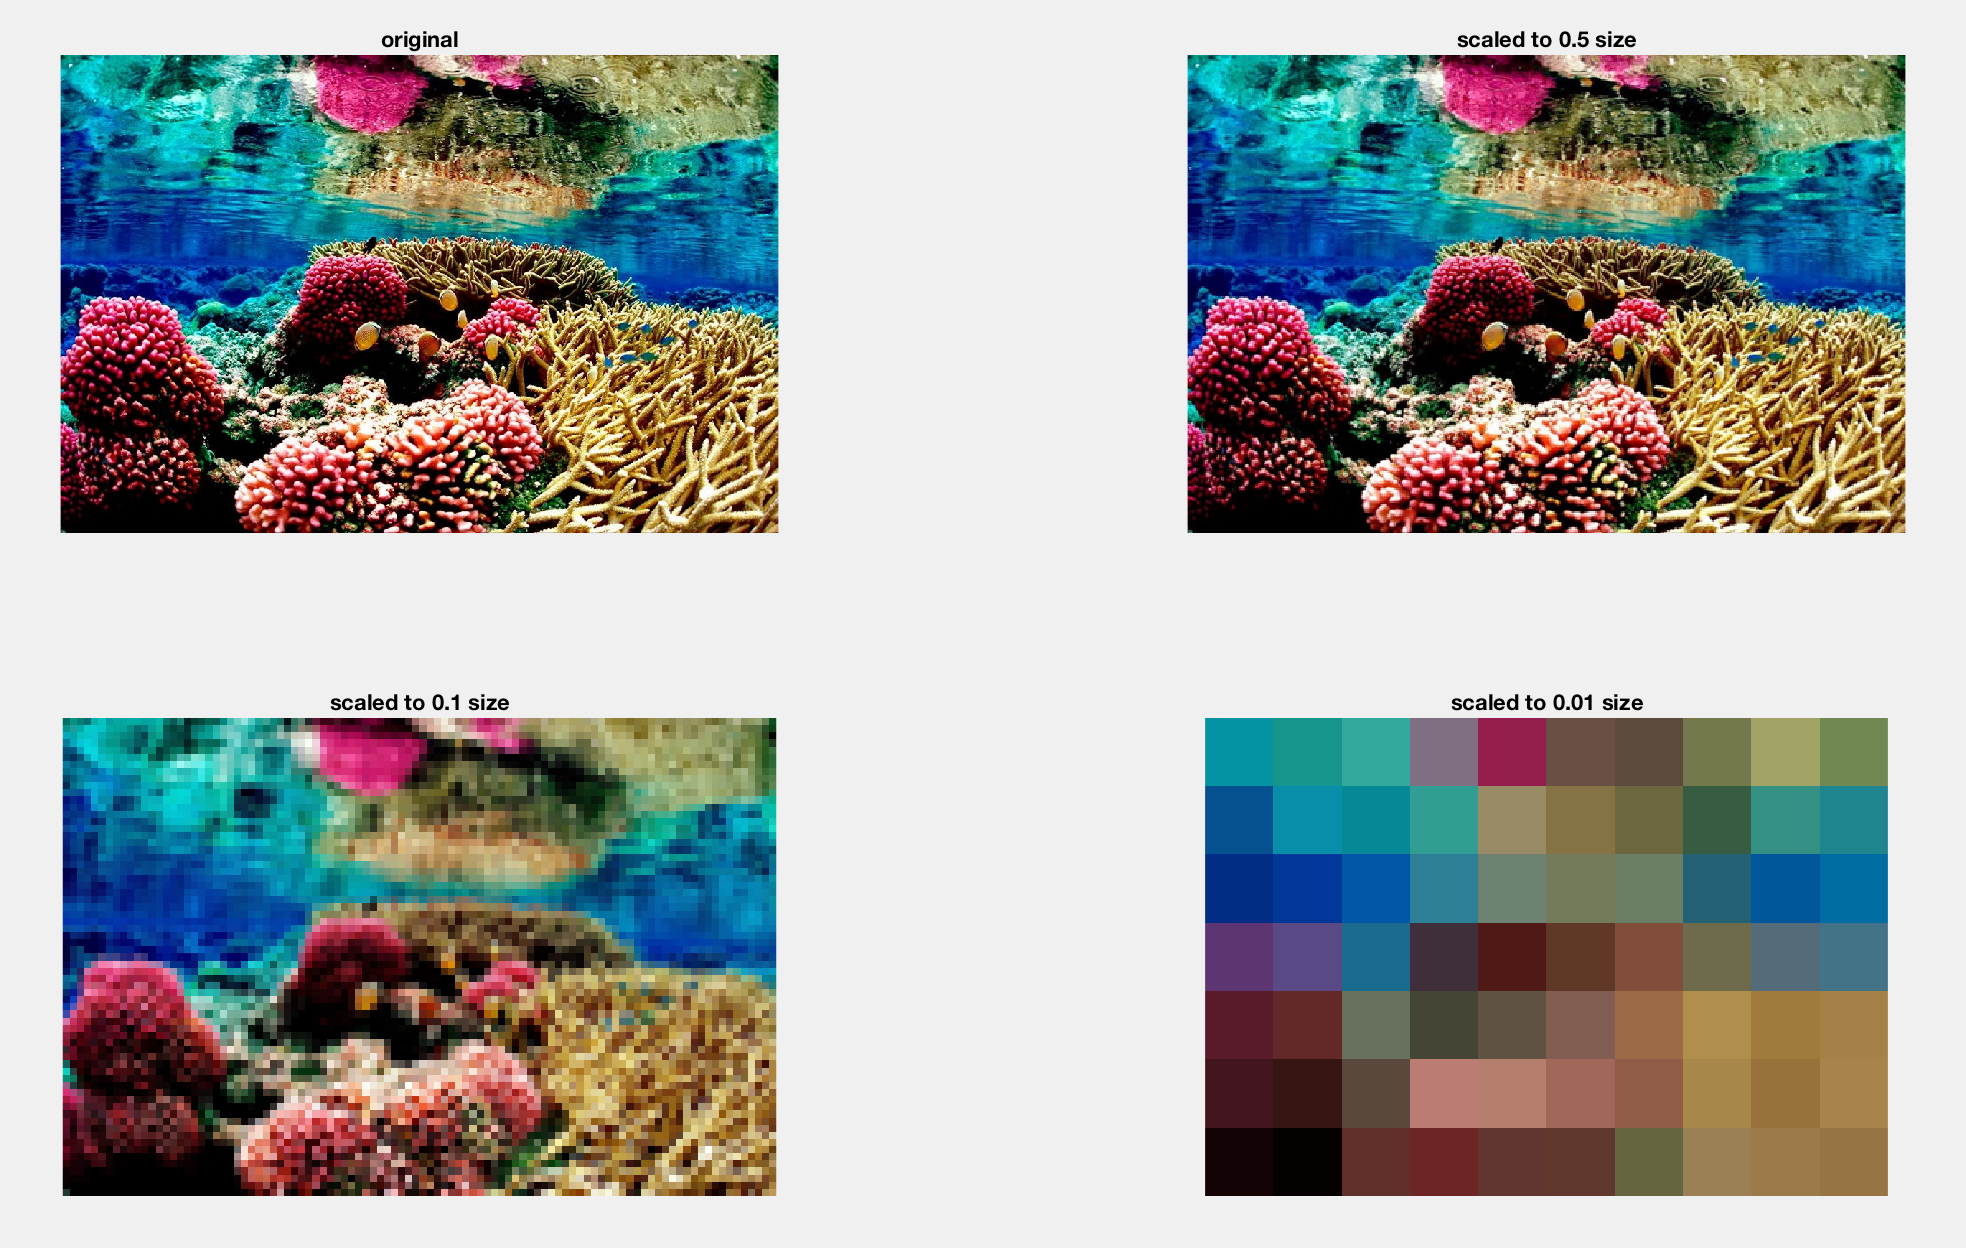
\includegraphics[width=\textwidth]{./img/task5.png}
  \caption{Resizing the original image to smaller sizes}
  \label{fig:task5}
\end{figure}

This loss of details after resizing can also be observed in the histogram of the three color channels. In figure \ref{fig:task6} the three histograms of the RGB-channels of the original image are shown in the left column. The same histograms are shown on the right, after reducing the size to 10\% of the original size. It can clearly be observed that after resizing, the channels' values are less smoothly distributed and are concentrated on a smaller number of distinct values. This is one of the effects of combining the values of several adjacent bins into one in order to allow a smaller size. 

\begin{figure}[!hbt]
  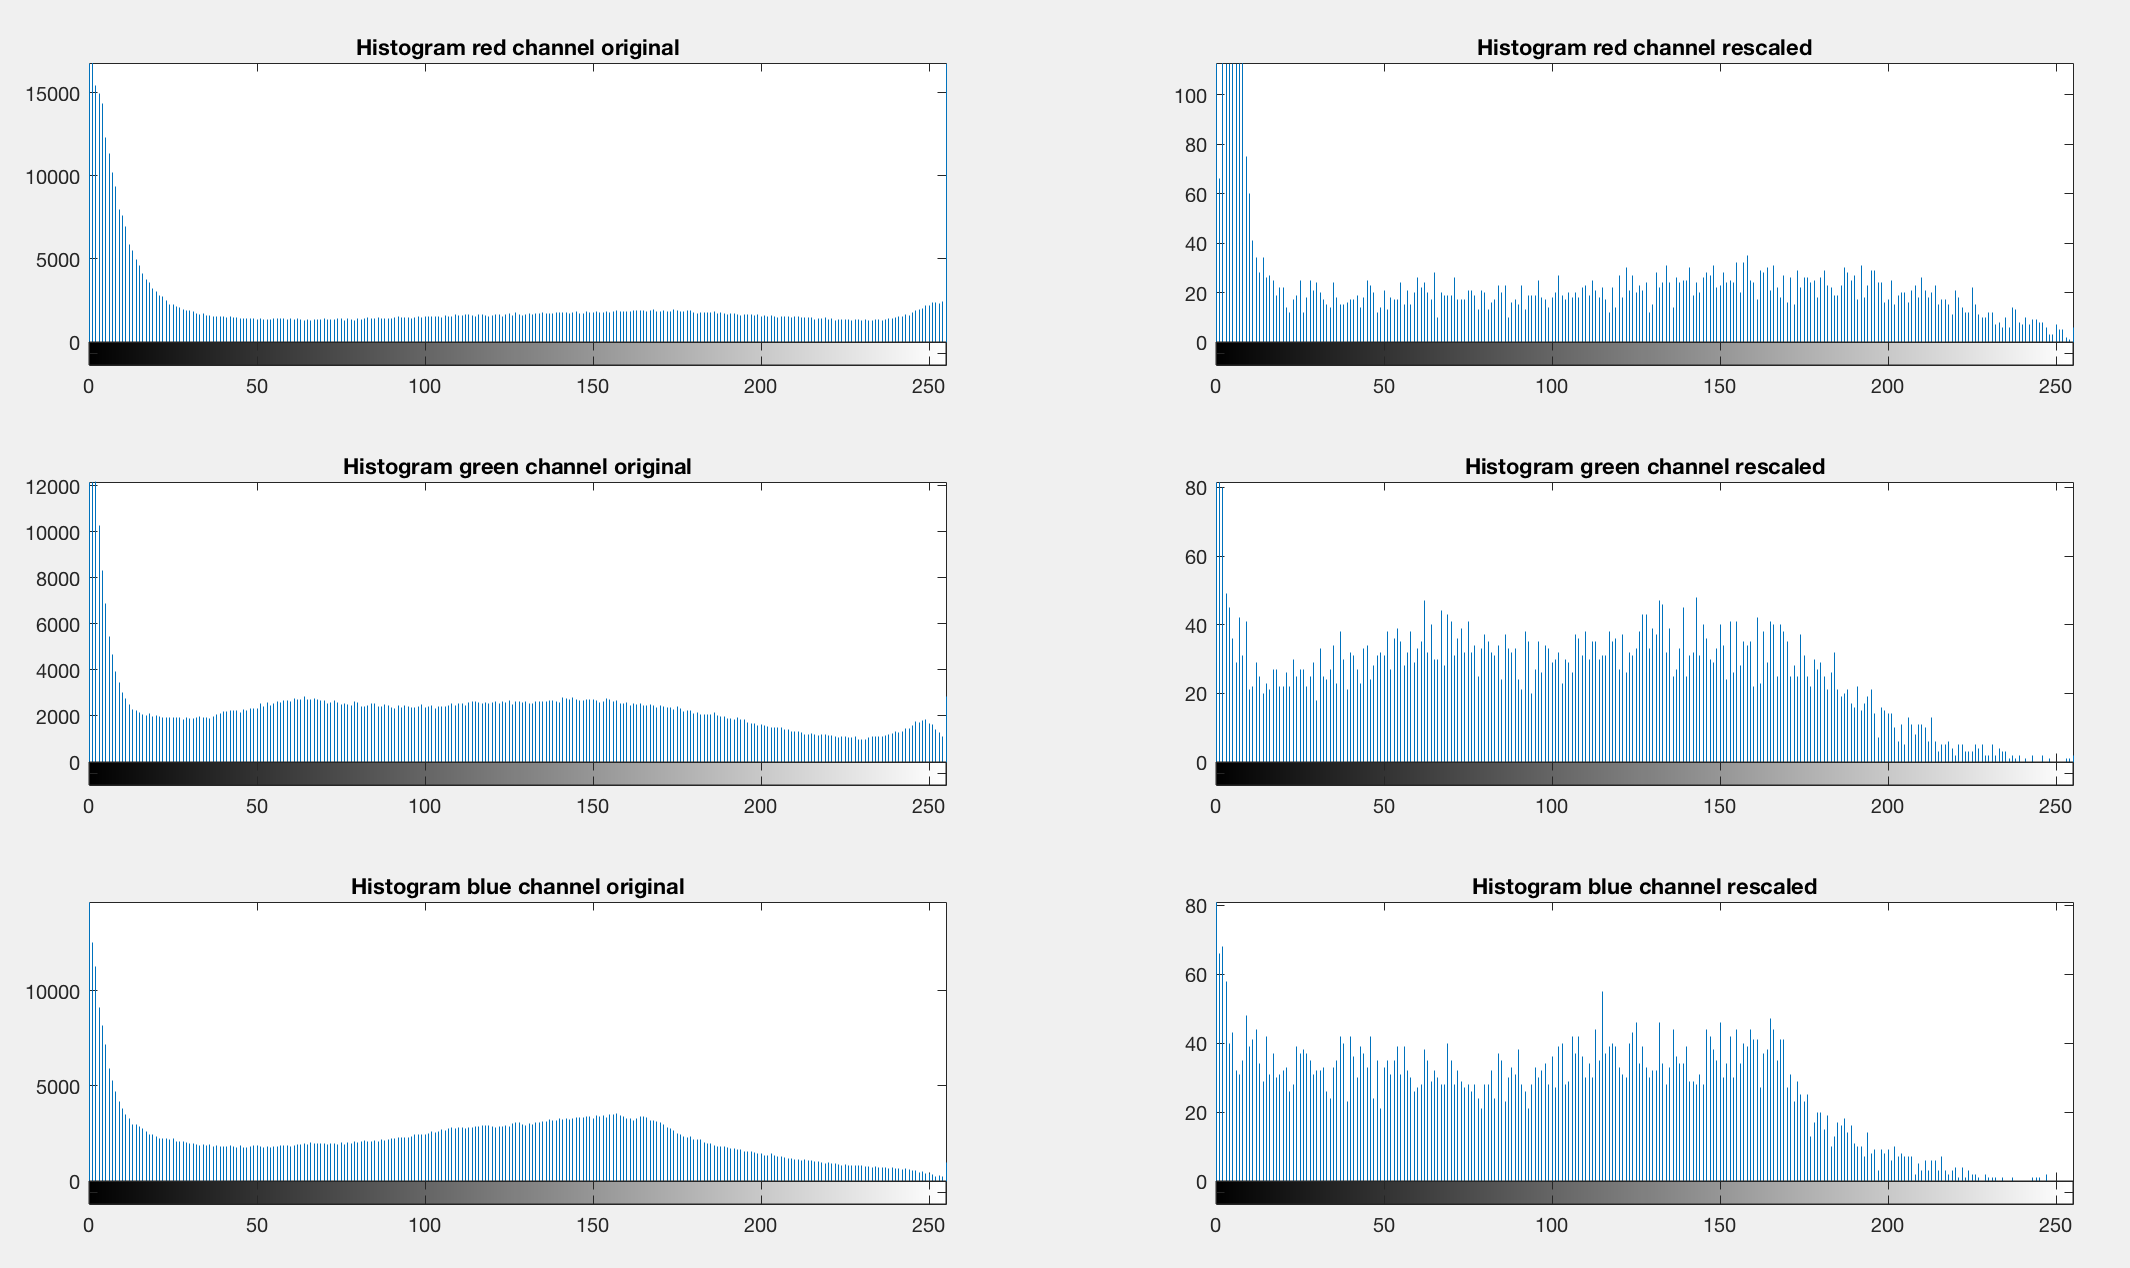
\includegraphics[width=\textwidth]{./img/task6.png}
  \caption{Change of the RGB histograms after resizing to 0.1 original size}
  \label{fig:task6}
\end{figure}

It is possible to return the smaller image back to its original size. As figure \ref{fig:task7} shows, the restored image keeps lacking the same amount of details of the original image. The details that were lost in the small image cannot be retrieved later. The only improvement is, that the restored image looks smoother and less pixelated, i.e. pixels boundaries are not perceptible with the same zoom factor as before. This is thanks to the bicubic interpolation method followed to scale the image back to its original size.

\begin{figure}[!hbt]
  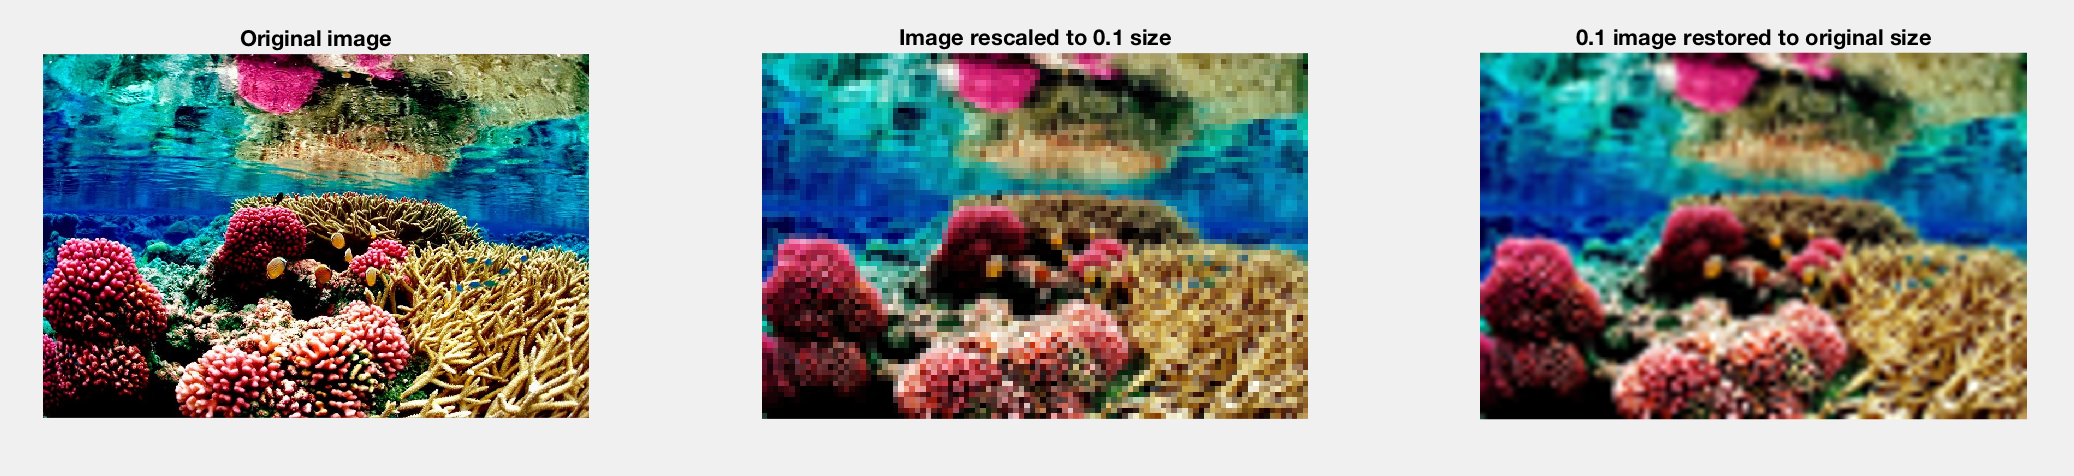
\includegraphics[width=\textwidth]{./img/task7.png}
  \caption{Resizing to 0.1 size and then restoring to original size}
  \label{fig:task7}
\end{figure}

This effect can be observed better when we zoom in a smaller area of the image, as in figure \ref{fig:task8}. This figure shows, that when scaling down to 0.1 of original size, most details are lost and the image looks very pixelated. When restoring the 0.1 image back to its original size with a bicubic interpolation, the pixelated look disappears, but the former details can not be recovered.

\begin{figure}[!hbt]
  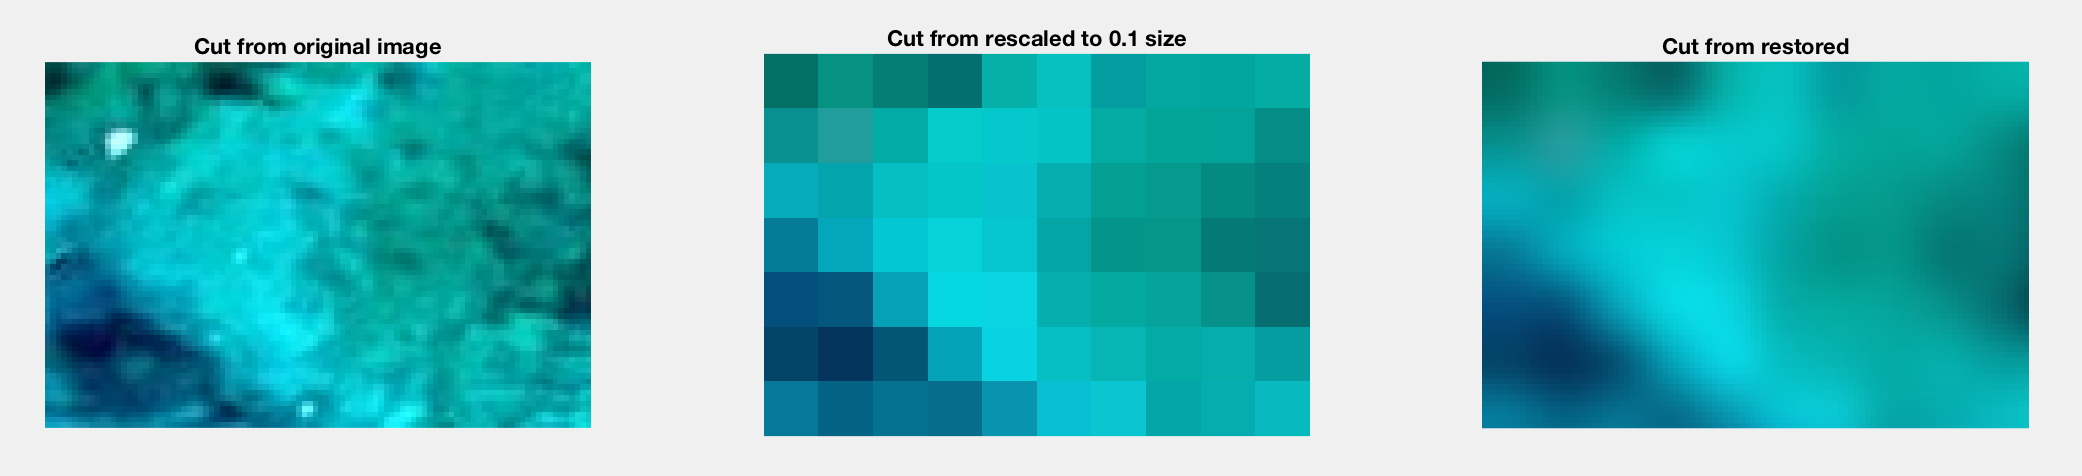
\includegraphics[width=\textwidth]{./img/task8.png}
  \caption{Resizing to 0.1 size and then restoring to original size (Zoomed in)}
  \label{fig:task8}
\end{figure}

As an alternative for removing image details different smoothing filters can be applied. One option is to apply evenly weighted moving averages that simply add all values in the neighborhood of a pixel and then normalize the sum by dividing through the number of added pixels. In this case, the size and shape of the area that is chosen to calculate the average has a big impact on the outcome, as can be seen in figures \ref{fig:task9} and \ref{fig:task10}.

In figure \ref{fig:task9} both a horizontal filter of size 1x50 pixel and a vertical filter of size 50x1 is applied to all pixels in the image. The former results in an effect that looks like the camera had been moving horizontally while taking the picture, while in the latter the movement is horizontal (this is known as motion blur in most photography/art suites like GIMP or Photoshop). While both filters will remove some kind of noise in the image or add some artistic effect, their results still look very different. 

\begin{figure}[!hbt]
  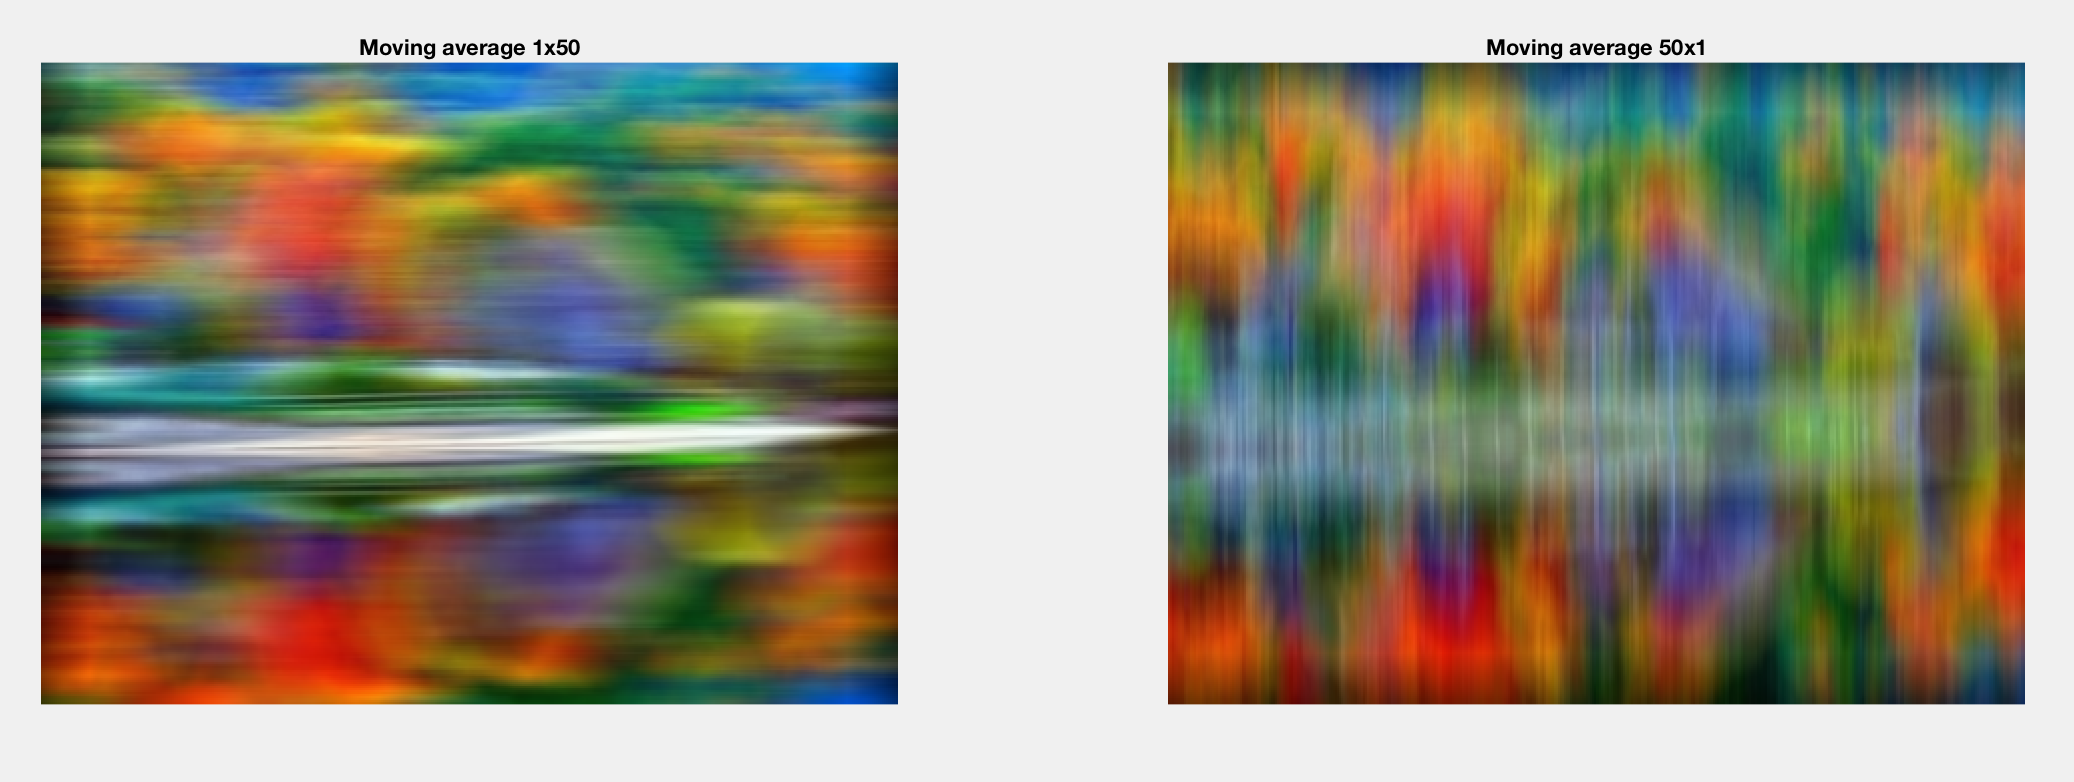
\includegraphics[width=\textwidth]{./img/task9.png}
  \caption{Horizontal and vertical evenly weighted moving average}
  \label{fig:task9}
\end{figure}

Figure \ref{fig:task10} shows evenly weighted moving average filters in square shape of different sizes from 3x3 to 100x100. The filter size determines how much noise is removed but also how many details are lost. Filters with a larger area make the image more blurry and remove more details, but they also have a greater denoising power. The optimal filter sizes can vary a lot from image to image.

\begin{figure}[!hbt]
  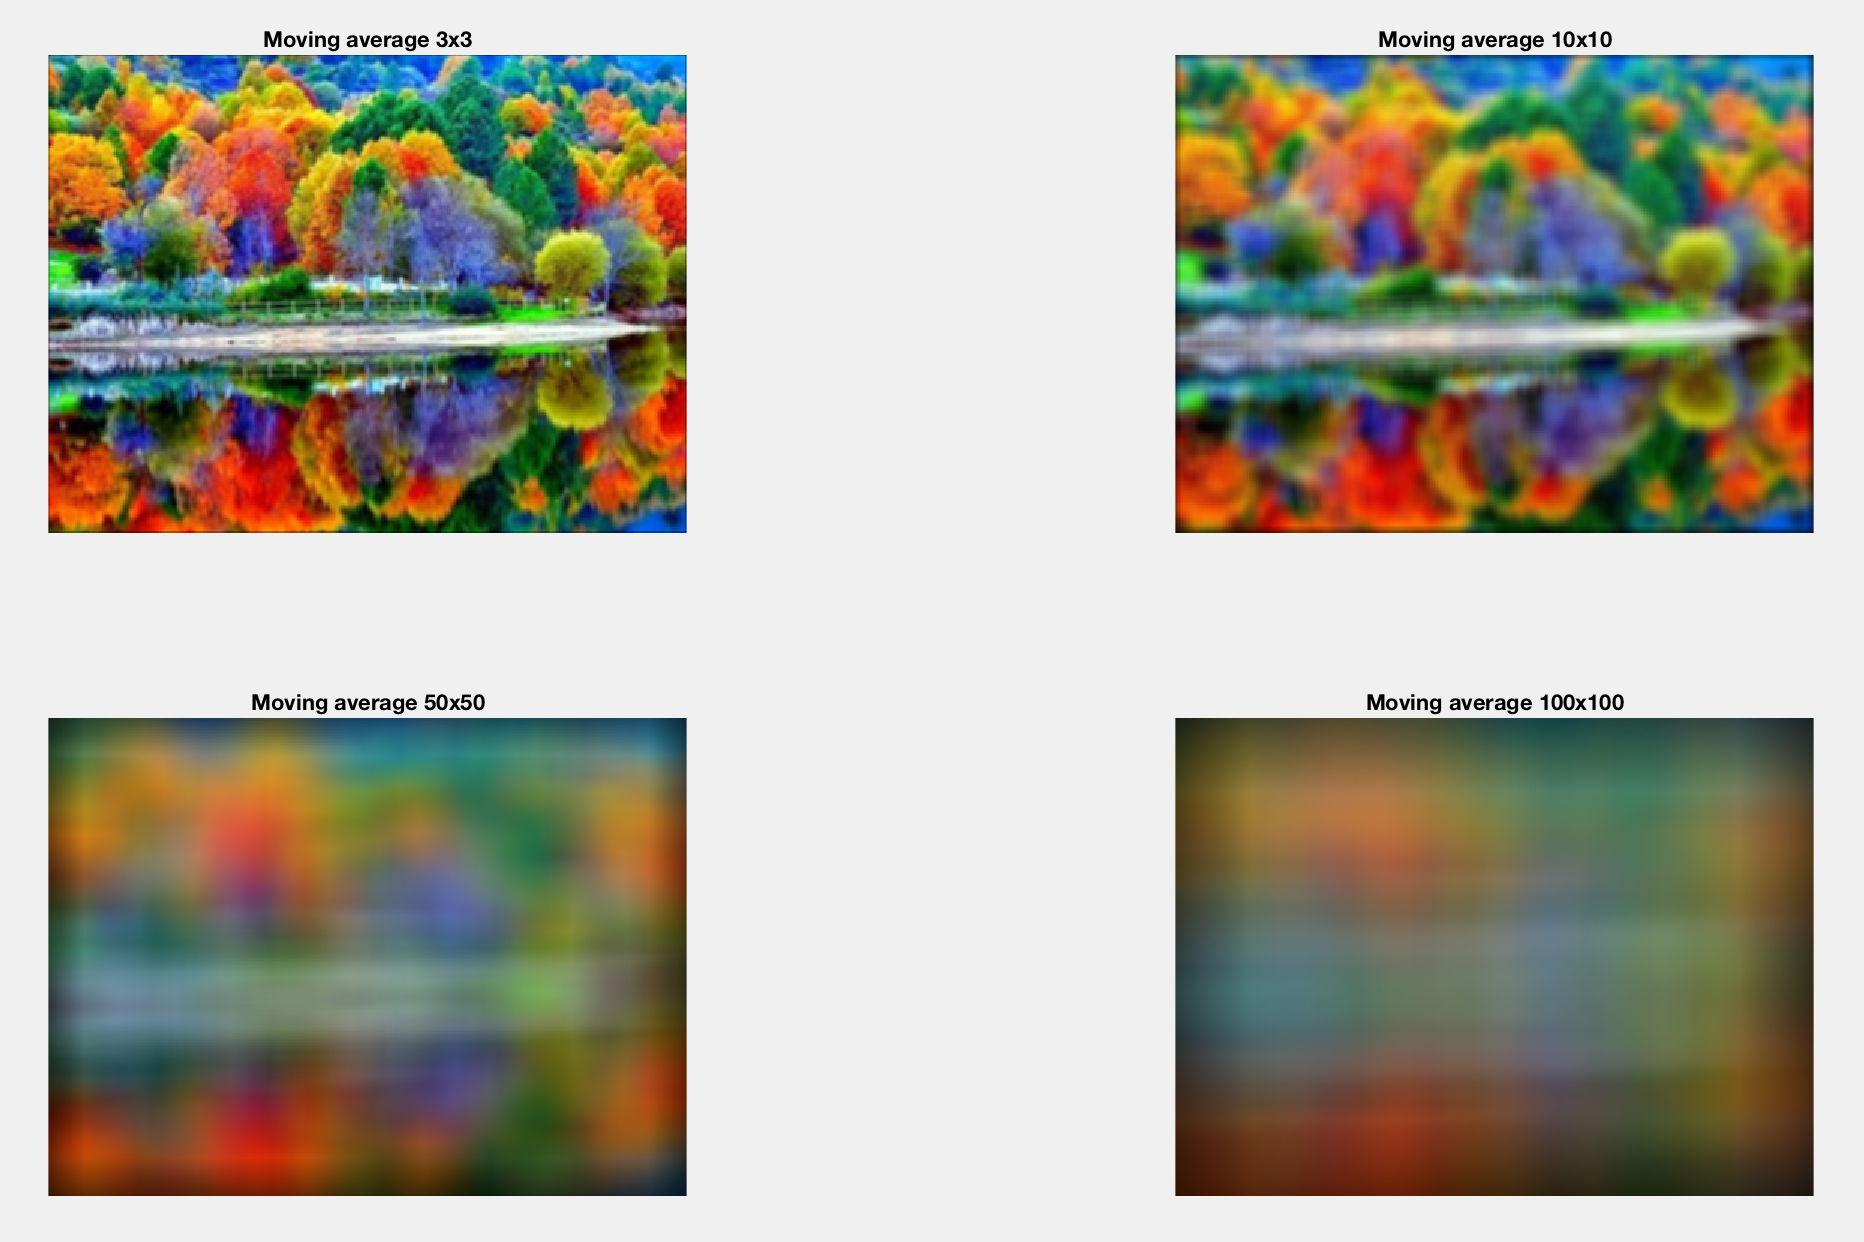
\includegraphics[width=\textwidth]{./img/task10.png}
  \caption{Square shaped evenly weighted moving averages in different sizes}
  \label{fig:task10}
\end{figure}

Besides evenly weighted moving averages it is also possible to reward proximity to the target pixel by weighting close neighbors of the pixel more highly. Figure \ref{fig:task11} shows the comparison of an evenly weighted horizontal kernel of 1 x 10 pixel size against a weighted horizontal kernel with weights [1, 2, 4, 8, 16, 32, 16, 8, 4, 2, 1]. The evenly weighted filtering gives the same importance to pixels that are much further away than close neighbors and results in a more blurry picture with less details.

\begin{figure}[!hbt]
  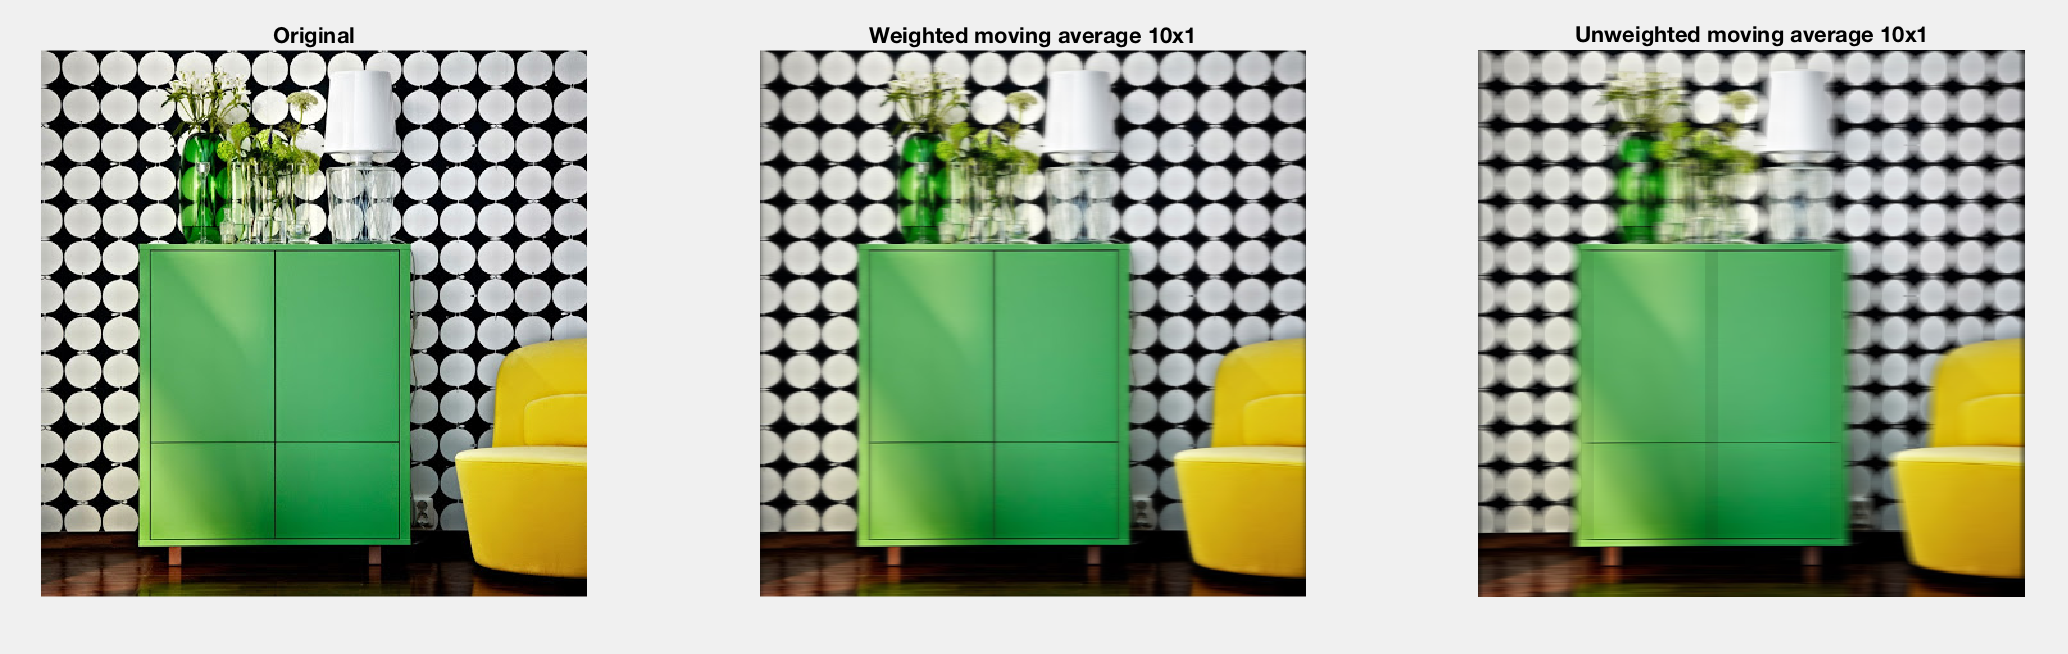
\includegraphics[width=\textwidth]{./img/task11.png}
  \caption{Weighted and evenly weighted horizontal moving average}
  \label{fig:task11}
\end{figure}

In several cases it is desired to weight neighbors closer to the target pixel higher than the ones that are further away. This can be achieved elegantly by applying a Gaussian kernel, like the ones depicted in figure \ref{fig:task12}. If the Gaussian filter is isotropic (i.e. same behavior in every direction), it has two parameters: kernel size and sigma. Otherwise, we would need to consider two additional parameters. The kernel size determines the maximum area in which pixels are considered to compute the filtered value of the target pixel. The value of sigma determines, how much stronger close neighbors are weighted, than distant neighbors. A small sigma results in close neighbors being weighted much higher than with a large sigma. It is very common to choose the kernel size as a function of sigma (e.g. three or five times sigma) to avoid having a prematurely truncated Gaussian kernel.

As a side note it is worth noticing that one of the main advantages of the ideal non-truncated Gaussian filter is the absence of side lobes in the frequency response. This is, it acts as a reasonably selective low-pass without oscillating behavior for high-frequency bands.

\begin{figure}[!hbt]
  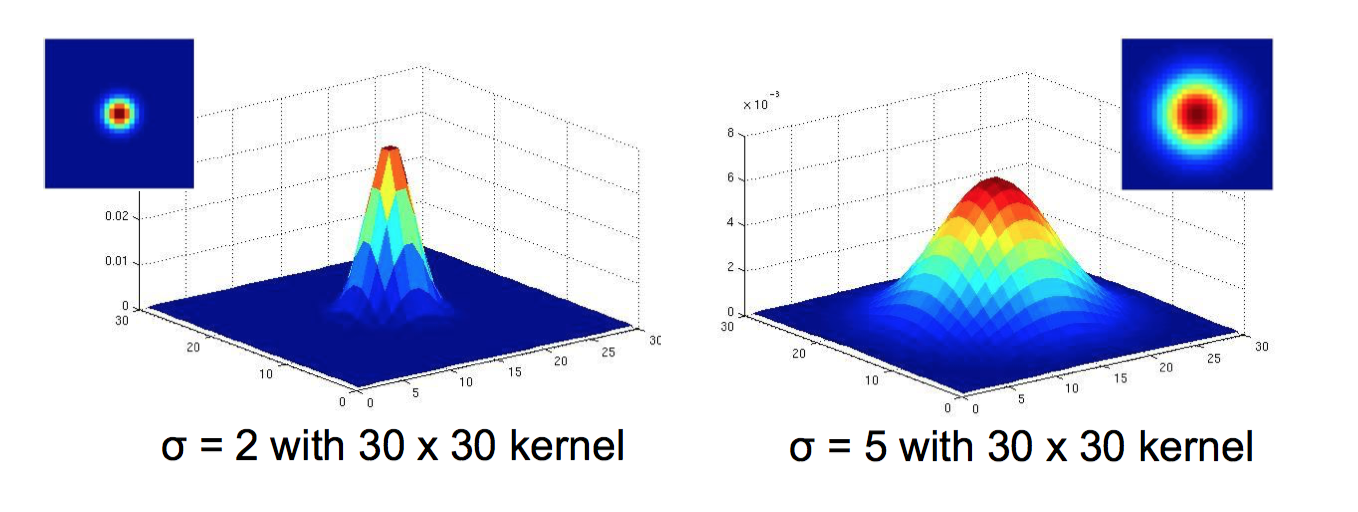
\includegraphics[width=\textwidth]{./img/task12.png}
  \caption{Two differently parametrized Gaussian kernels}
  \label{fig:task12}
\end{figure}

Figure \ref{fig:task13} shows the effect of different kernel sizes of a Gaussian filter. The left image used a kernel with area 10x10 pixels and the right image with a kernel of 30x30 pixels is clearly more blurry with more details and noise removed. This is because the 10x10 kernel is a prematurely truncated sigma.

\begin{figure}[!hbt]
  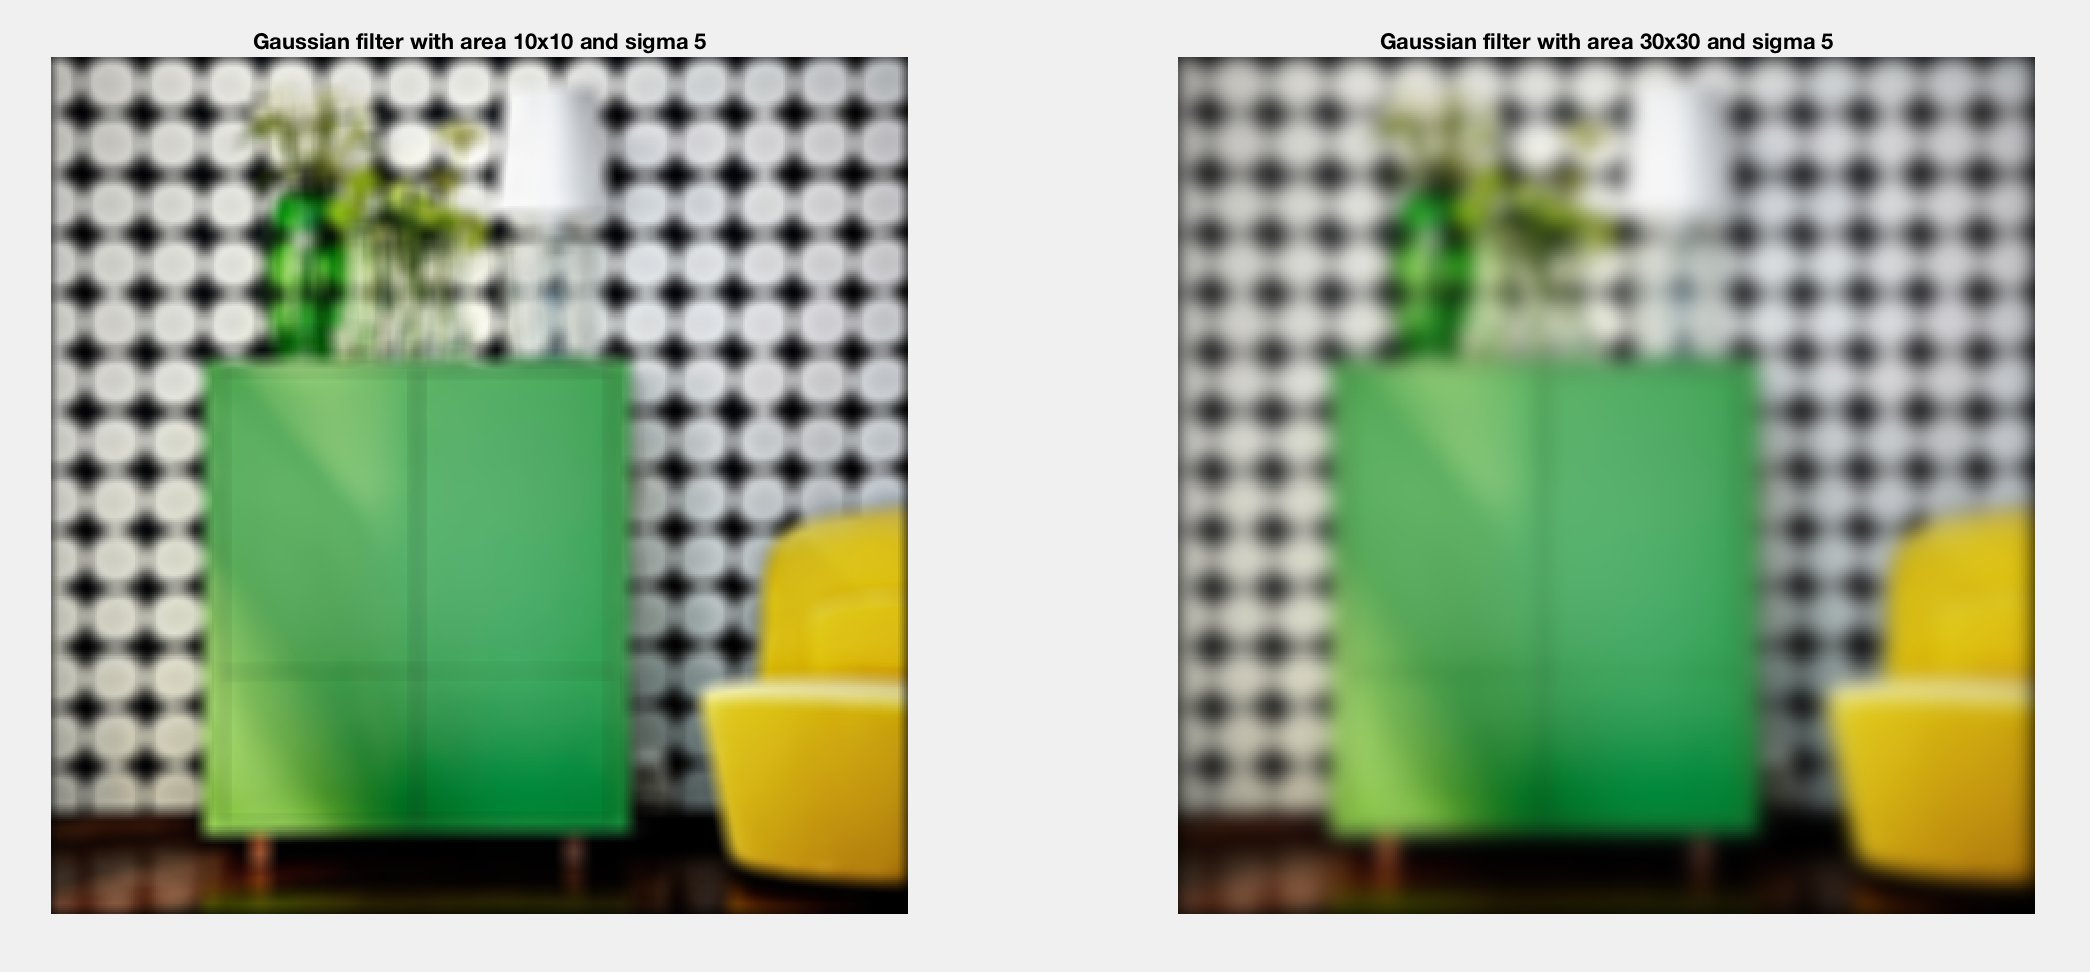
\includegraphics[width=\textwidth]{./img/task13.png}
  \caption{Gaussian kernels with different areas}
  \label{fig:task13}
\end{figure}

As described before, the choice of sigma for Gaussian kernels also influences their effect. This can be seen in figure \ref{fig:task14}.

\begin{figure}[!hbt]
  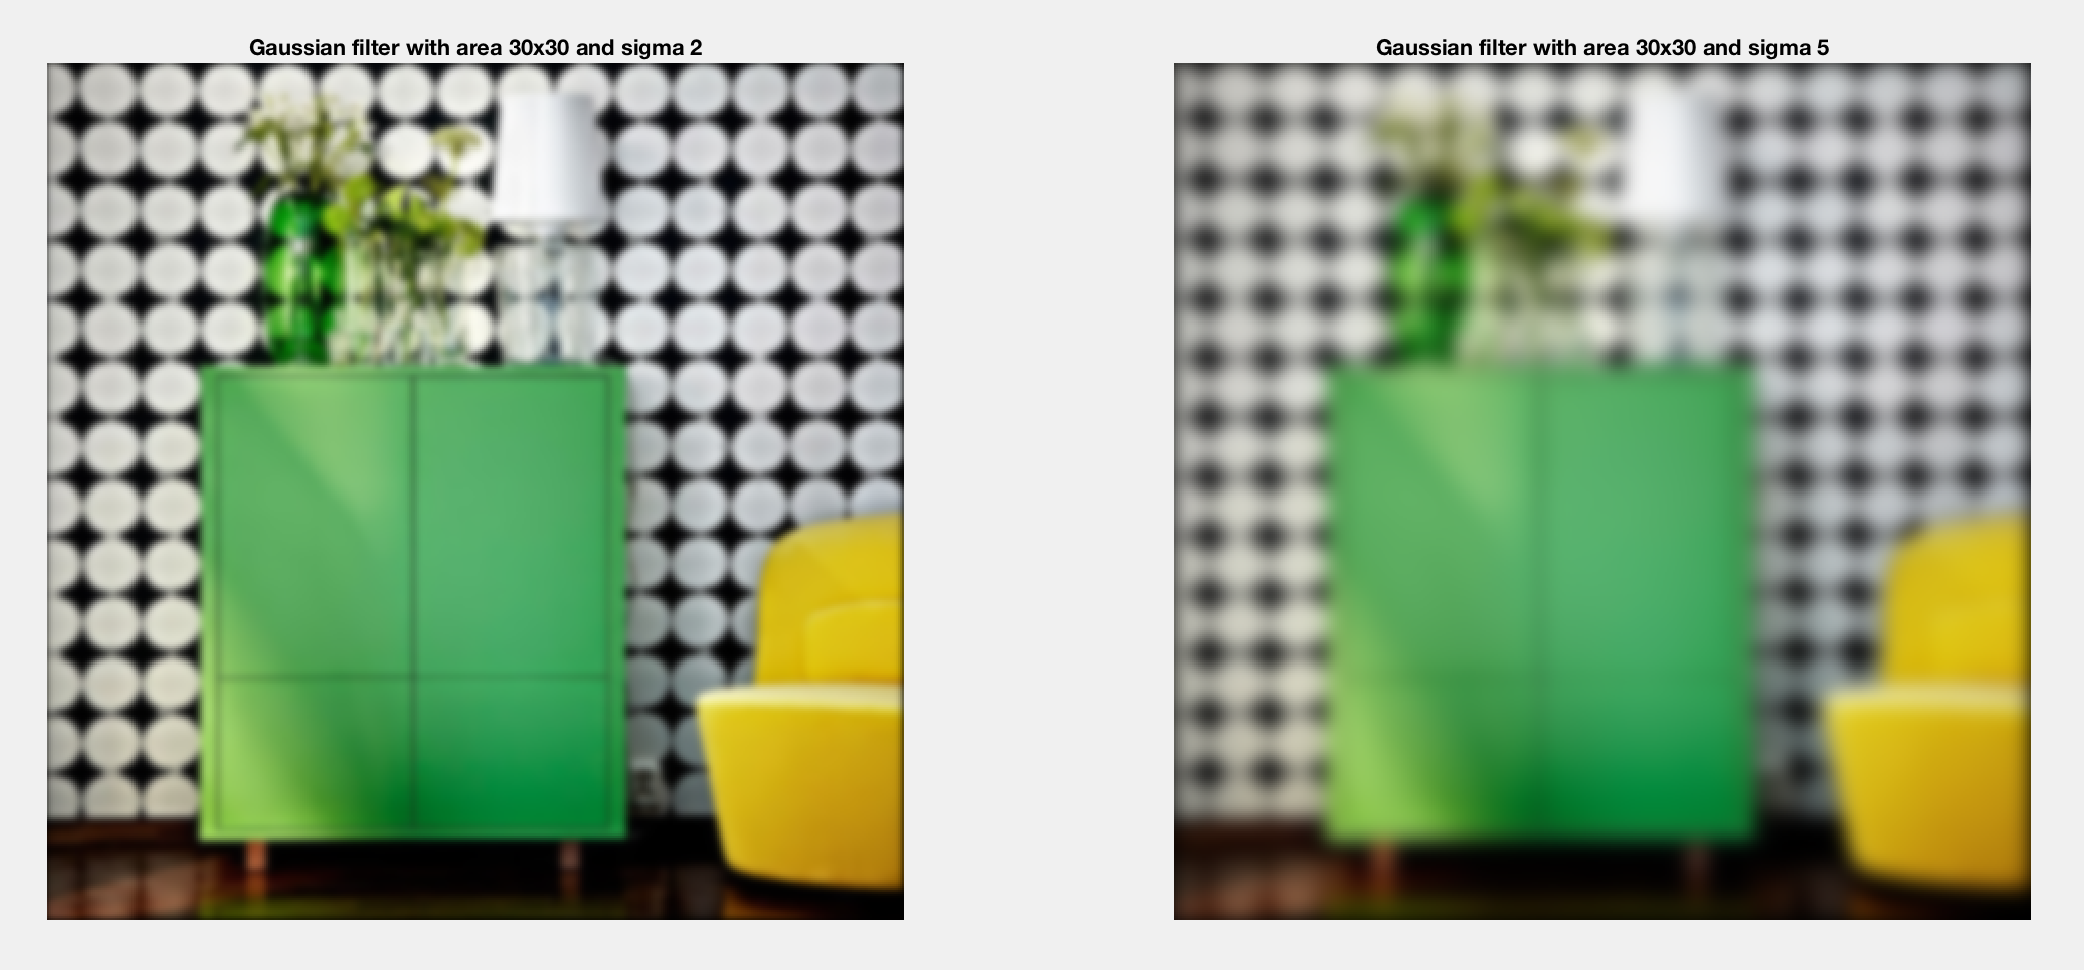
\includegraphics[width=\textwidth]{./img/task14.png}
  \caption{Gaussian kernels with different sigmas}
  \label{fig:task14}
\end{figure}

The built-in function \textit{imfilter} in Matlab can use both custom filters like the weighted average and predefined filters like the Gaussian on both RGB and gray scale images. Even though the kernel is 2-dimensional, the function can apply it sequentially and independently on all three channels of the three-dimensional RGB-images.

Usually it is desired to normalize kernels in convolution filtering in order to keep the values of the resulting image bounded. If the filter is not normalized, the output is very likely to saturate. This effect can be seen in figure \ref{fig:task15}.

\begin{figure}[!hbt]
  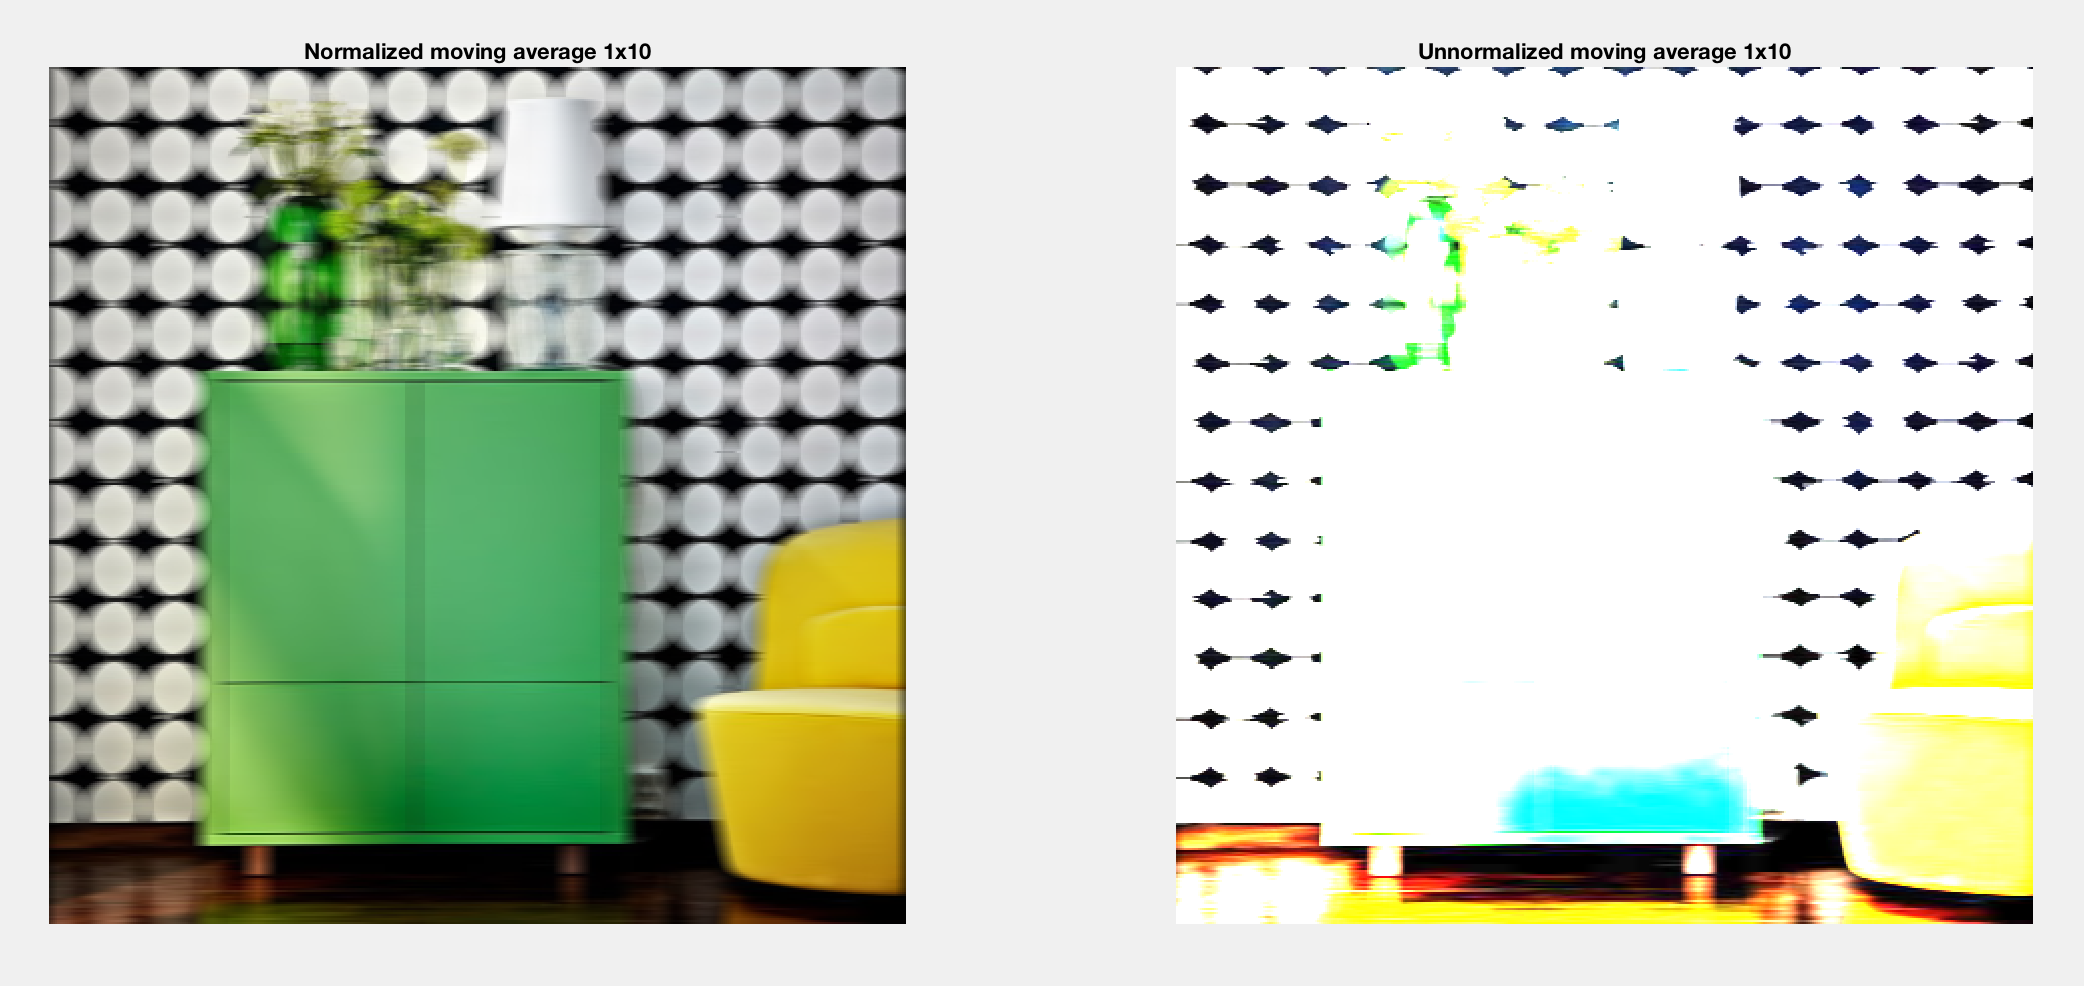
\includegraphics[width=\textwidth]{./img/task15.png}
  \caption{The importance of normalizing kernels}
  \label{fig:task15}
\end{figure}

It is also possible to apply the same filter iteratively more than once to an image. The effect can be observed in figure \ref{fig:task16}. It is worth noticing that convolving more than once an image with the same kernel will be similar to applying an Gaussian filter (anisotropic in the general case) from the beginning. This is because of the central limit theorem (we can think of convolving the same filter with itself several time as summing several identically distributed random variables).

\begin{figure}[!hbt]
  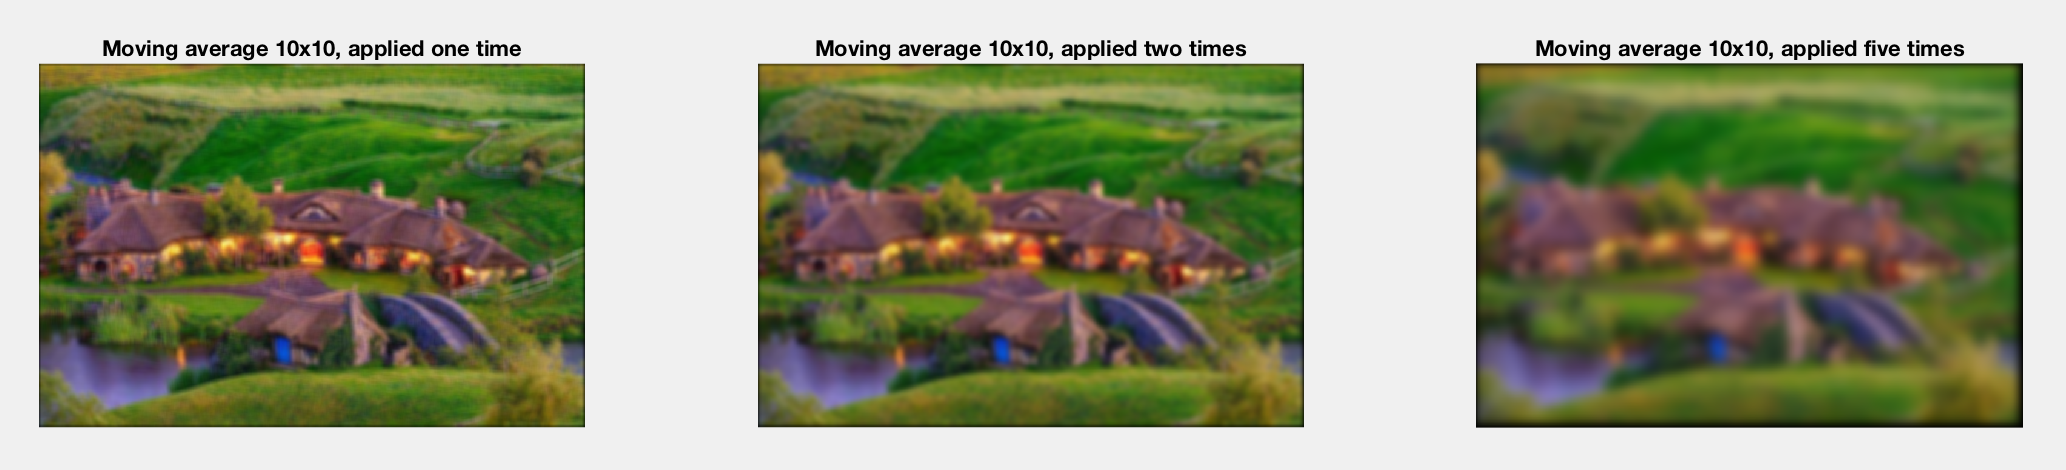
\includegraphics[width=\textwidth]{./img/task16.png}
  \caption{Applying filters multiple times}
  \label{fig:task16}
\end{figure}

When calculating the absolute difference between a smoothed image and its original, we get an effect similar to that in figure \ref{fig:task17}. Areas of the image that have very similar pixel values in both images look darker (near zero values) on the difference image. Only in areas of the image where pixels change more drastically, the difference shows higher values. This can be seen as an idea for an edge detection technique. In fact, DoG (Difference of Gaussians) is a well known algorithm for edge detection which puts into practice a similar concept.

\begin{figure}[!hbt]
  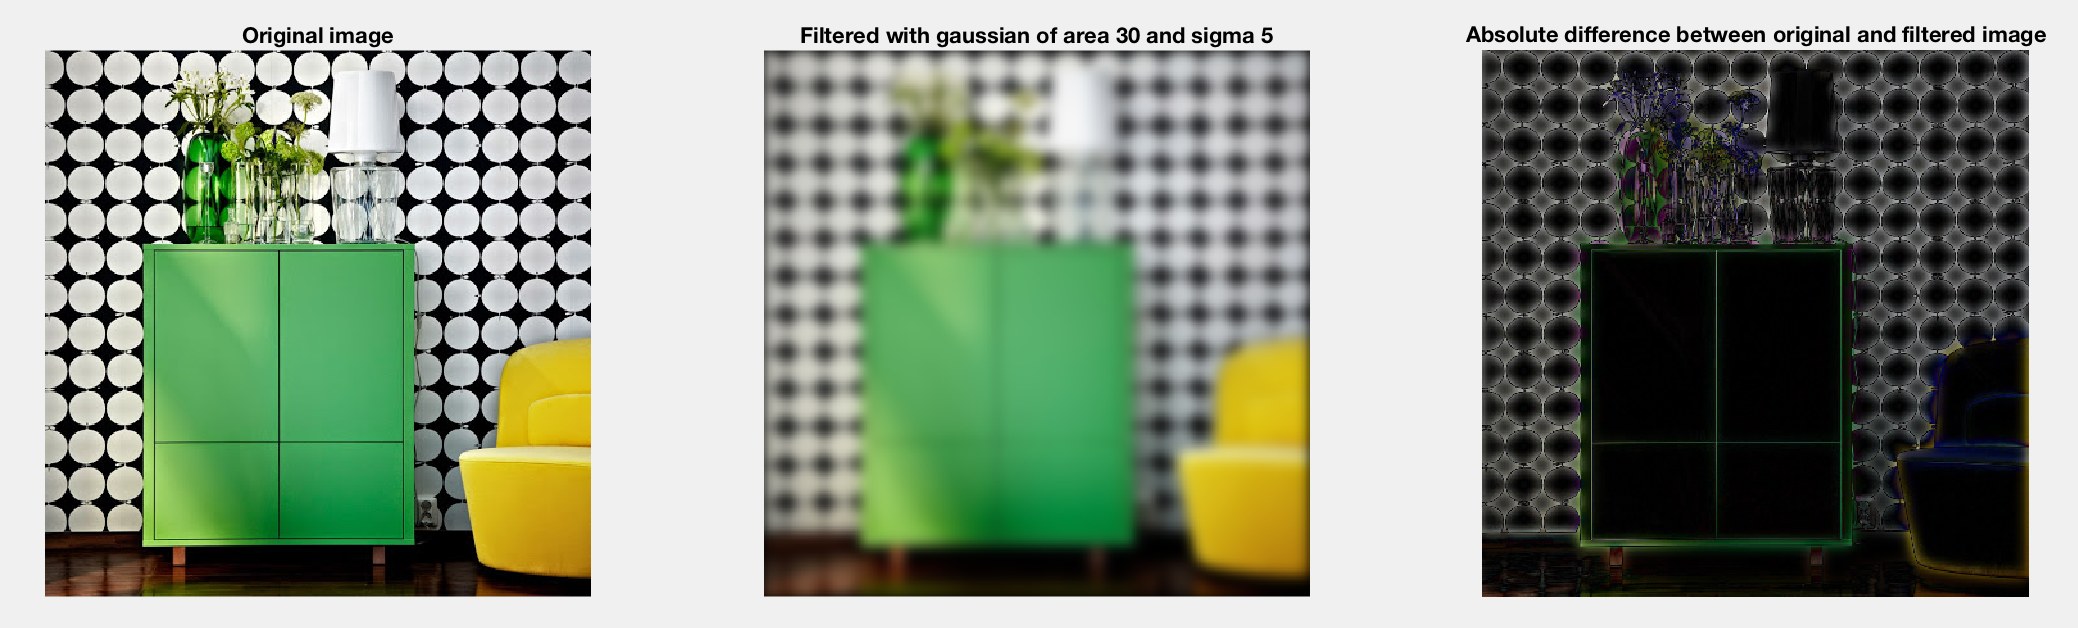
\includegraphics[width=\textwidth]{./img/task17.png}
  \caption{Absolute difference between a smoothed image and its original}
  \label{fig:task17}
\end{figure}
